\documentclass[11pt,a4paper]{article}
\usepackage[T1]{fontenc}
\usepackage[utf8]{inputenc}
\usepackage{lmodern}
\usepackage[margin=2.3cm]{geometry}
\usepackage{amsmath,amssymb,bm}
\usepackage{graphicx}
\usepackage{booktabs}
\usepackage{array}
\usepackage{multirow}
\usepackage{xcolor}
\usepackage{caption}
\usepackage{subcaption}
\usepackage{tikz}
\usetikzlibrary{positioning,arrows.meta,calc,decorations.pathreplacing,shapes.geometric,fit,backgrounds}
\usepackage{listings}
\usepackage{enumitem}
\usepackage[hidelinks]{hyperref}
\usepackage{microtype}
\usepackage{placeins}

\definecolor{sfred}{HTML}{C8102E}
\definecolor{sfblue}{HTML}{2E5090}
\definecolor{sfgrey}{HTML}{5A5A5A}
\definecolor{sfgreen}{HTML}{2A8C55}
\definecolor{sforange}{HTML}{E07B00}
\definecolor{sflight}{HTML}{F2F4F8}

\lstset{basicstyle=\ttfamily\small,breaklines=true,columns=fullflexible,frame=single,framerule=0.3pt,rulecolor=\color{sfgrey},backgroundcolor=\color{sflight},xleftmargin=4pt}
\captionsetup{font=small,labelfont=bf}
\graphicspath{{figs/}}
\setlist{nosep}

\newcommand{\tool}{\texttt{ascentopt}}
\newcommand{\dv}{\Delta v}
\newcommand{\unit}[1]{\,\mathrm{#1}}

\title{\textbf{\tool: a launch-trajectory / propulsion co-design tool}\\[4pt]
\large Modeling approach, verification, and a Starship Block~3 example\\[2pt]
\normalsize MECE~4305 Mechanics \& Thermodynamics of Propulsion --- Rocket module, Fall 2026}
\author{D.~E.~Tew (Columbia University) with Claude\\ \small prototype v0.1, 9~November 2026}
\date{}

\begin{document}
\maketitle

\begin{abstract}
\noindent\tool\ replaces the prescribed-steering forward simulation shown on Week~9 slide~33 with a
multi-phase direct-collocation optimizer built on Dymos/OpenMDAO: the same 3-DOF point-mass physics, but
thrust direction and throttle are solved for, staging is a phase linkage, orbit insertion is a constraint
and payload is the objective. Vehicle parameters (stage propellant loads, dry masses, reserves, engines) are
an input deck that can be swept now and optimized in the same problem in the next milestone. This report
documents the model, the numerical method, the verification performed, and a worked example: SpaceX
Starship/Super~Heavy Block~3 to a $275\unit{km}\times26^\circ$ orbit from Starbase. With published propellant loads,
Raptor~3 performance and the slide-42 mid-range dry masses (200/100~t), the optimizer places
\textbf{293.3~t} in orbit on an expendable trajectory with losses of 1.83~km/s; holding back 8\,\% of the
booster propellant for boost-back and 30~t in the ship for landing reduces this to 204.5~t, and the ship's dry
mass trades against payload exactly 1:1. The results are grid-independent to 0.04\,\%, re-integrate explicitly
to within 211~m and 4.5~m/s, and close the slide-28 $\dv$ identity to 1~mm/s.
\end{abstract}

\section{Why a trajectory optimizer}
\label{sec:why}

The Week~9 lecture closed the mission-analysis block with a rule of thumb: $\dv_{\mathrm{LEO}} \approx v_{\mathrm{circ}}
+ \dv_{\mathrm{loss}} - v_{\mathrm{rot}} \approx 9.3\unit{km/s}$ with $\dv_{\mathrm{loss}} = 1.5$--$2.0\unit{km/s}$ (slides 28 and 32),
and with a forward simulation of a gravity turn (slide~33) that arcs to 250~km and falls back. Both are correct as
far as they go, and neither can answer the questions the design project asks:
\begin{itemize}
  \item How much payload does a \emph{given} two-stage vehicle deliver to a \emph{given} orbit, and where should it stage?
  \item How large are the gravity, drag, steering and back-pressure losses \emph{for this vehicle}, rather than as a band?
  \item How much does each kilogram of booster dry mass, ship dry mass or return propellant cost in payload?
  \item What thrust, $I_{sp}$, chamber pressure and burn time must the propulsion system deliver --- the inputs to
        thrust-chamber and cycle design (Week~12 design-procedure steps 6--9)?
\end{itemize}
Table~\ref{tab:tsiolkovsky} shows the size of the problem with the hand method. The rocket equation with the
Starship deck of Section~\ref{sec:example} returns anywhere from 276 to 339~t of payload depending on where in the
1.5--2.0~km/s loss band one lands; with the \emph{actual} $\dv$ requirement from the optimized trajectory it
returns 293.3~t, identically the optimizer's answer. The trajectory tool does not change the physics --- it
removes the assumption.

\begin{table}[h]\centering\footnotesize
\caption{Rocket-equation closure for the Starship Block~3 deck (vacuum $I_{sp}$ 350.0/363.9~s, dry 200/100~t)
versus the assumed $\dv$ requirement. The optimizer's requirement for this vehicle and orbit is 9,155~m/s.}
\label{tab:tsiolkovsky}
\begin{tabular}{lccc}
\toprule
Assumed $\dv_{\mathrm{req}}$ [m/s] & Loss assumption & Payload, no reserves [t] & Payload, 292/30~t reserves [t] \\
\midrule
8,800 & 1.5~km/s & 339.0 & 250.6 \\
9,300 & 2.0~km/s (+ margin) & 276.2 & 195.7 \\
\textbf{9,155} & \textbf{optimizer: 1,833~m/s} & \textbf{293.3} & 210.7$^{\dagger}$ \\
\midrule
\multicolumn{2}{l}{\tool\ (trajectory optimized)} & \textbf{293.3} & \textbf{204.5} \\
\bottomrule
\end{tabular}\\[2pt]
{\footnotesize $^{\dagger}$ the reserve case has its own optimal trajectory with 1,876~m/s of losses; the hand method cannot know that.}
\end{table}

\section{What the tool is}
\label{sec:what}

Figure~\ref{fig:pipeline} shows the workflow. A YAML vehicle deck and a mission definition are turned into a
Dymos \texttt{Trajectory} (one phase per burn, linked in time and state); the Week~9 notebook's own
gravity-turn law provides the initial guess; IPOPT solves the resulting sparse nonlinear program; the
optimized controls are re-integrated with an explicit integrator as a check; and the outputs are the time
histories of slide~33 plus staging state, loss breakdown, and the propulsion requirements for the next design
steps. Table~\ref{tab:compare} compares the capabilities with the notebook.

\begin{figure}[h]\centering
\resizebox{\textwidth}{!}{%
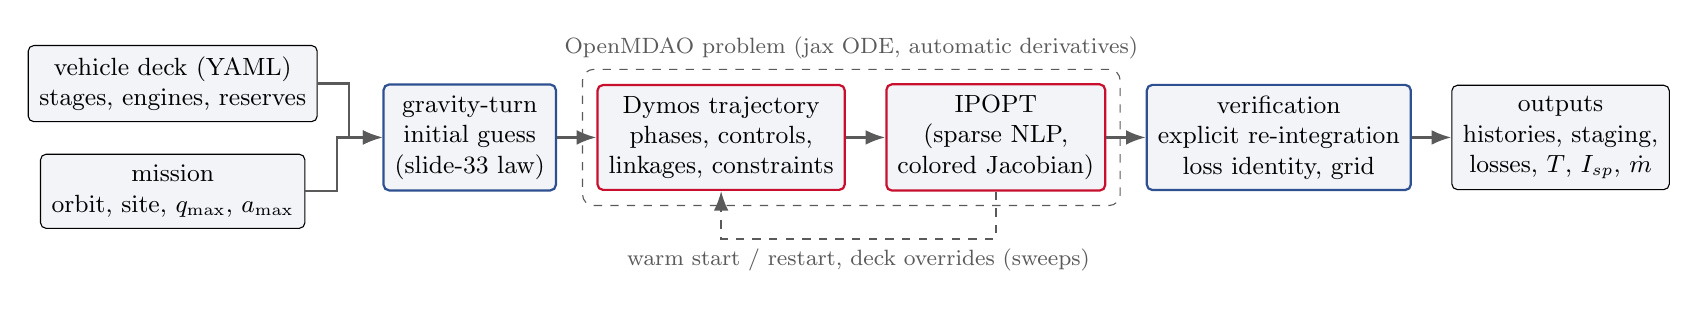
\begin{tikzpicture}[node distance=4mm and 5mm, font=\small,
  box/.style={draw, rounded corners=2pt, align=center, minimum height=9mm, inner sep=4pt, fill=sflight},
  red/.style={box, draw=sfred, thick}, blue/.style={box, draw=sfblue, thick},
  arr/.style={-{Latex[length=2.5mm]}, thick, sfgrey}]
  \node[box] (deck) {vehicle deck (YAML)\\stages, engines, reserves};
  \node[box, below=of deck] (mis) {mission\\orbit, site, $q_{\max}$, $a_{\max}$};
  \node[blue, right=9mm of $(deck.east)!0.5!(mis.east)$] (guess) {gravity-turn\\initial guess\\(slide-33 law)};
  \node[red, right=of guess] (nlp) {Dymos trajectory\\phases, controls,\\linkages, constraints};
  \node[red, right=of nlp] (ipopt) {IPOPT\\(sparse NLP,\\colored Jacobian)};
  \node[blue, right=of ipopt] (ver) {verification\\explicit re-integration\\loss identity, grid};
  \node[box, right=of ver] (out) {outputs\\histories, staging,\\losses, $T$, $I_{sp}$, $\dot m$};
  \draw[arr] (deck.east) -- ++(4mm,0) |- (guess.west);
  \draw[arr] (mis.east) -- ++(4mm,0) |- (guess.west);
  \draw[arr] (guess) -- (nlp); \draw[arr] (nlp) -- (ipopt); \draw[arr] (ipopt) -- (ver); \draw[arr] (ver) -- (out);
  \draw[arr, dashed] (ipopt.south) -- ++(0,-6mm) -| node[pos=0.25, below, font=\footnotesize]{warm start / restart, deck overrides (sweeps)} (nlp.south);
  \begin{scope}[on background layer]
    \node[draw=sfgrey, dashed, rounded corners, fit=(nlp)(ipopt), inner sep=5pt, label={[font=\footnotesize, sfgrey]above:OpenMDAO problem (jax ODE, automatic derivatives)}] {};
  \end{scope}
\end{tikzpicture}}
\caption{Workflow of \tool. The two existing pieces of the course --- the slide-33 integrator and the Week~12 design procedure --- bracket the optimizer: the former supplies the guess and an independent check, the latter consumes the outputs.}
\label{fig:pipeline}
\end{figure}

\begin{table}[h]\centering\small
\caption{Capability comparison with the Week~9 slide-33 notebook (\texttt{LaunchTrajectoryAnalysis.ipynb}).}
\label{tab:compare}
\begin{tabular}{p{4.2cm}p{5.2cm}p{5.8cm}}
\toprule
 & Slide-33 notebook & \tool\ v0.1 \\
\midrule
Dynamics & 3-DOF point mass, spherical coordinates & 3-DOF point mass, ECI Cartesian (no polar singularity) \\
Earth rotation & initial velocity $\omega R\cos\phi$ & $\bm v_0 = \bm\omega\times\bm r_0$; drag on air-relative velocity \\
Atmosphere & \texttt{ambiance} ISA to 81~km & US76 to 1000~km, smooth, differentiable \\
Engines & $I_{sp}$ linear in $p_a/p_{SL}$ & $T(h)=\tau(T_{vac}-p_aA_e)$ from one anchor + exit area \\
Steering & prescribed gravity turn & solved for: unit vector $\bm u(t)$ and throttle $\tau(t)$ \\
Stages & one & any number, phase per stage, propellant state per stage \\
Constraints & none & $q\le q_{\max}$, $T/m\le a_{\max}$, $h\ge0$, throttle bounds, orbit insertion \\
Objective & none (simulation) & max payload / min propellant / min time \\
Loss budget & --- & five accumulator states; slide-28 identity closed numerically \\
Verification & --- & explicit re-integration, grid independence, benchmark (Longuski SSTO) \\
Run time & seconds & 2--4~min per case (IPOPT, 16 Radau segments per phase, laptop-class CPU) \\
\bottomrule
\end{tabular}
\end{table}

\section{Physical model}
\label{sec:model}

\subsection{Equations of motion}
The vehicle is a point mass in an Earth-centered inertial frame (Figure~\ref{fig:forces}). With position $\bm r$,
inertial velocity $\bm v$, propellant mass of the active stage $m_p$, and total mass
$m = m_p + m_{\mathrm{struct}} + m_{\mathrm{pay}}$ (structure of the active stage plus everything above it),
\begin{align}
\dot{\bm r} &= \bm v, \\
\dot{\bm v} &= -\frac{\mu}{|\bm r|^3}\bm r + \frac{T}{m}\,\hat{\bm u} - \frac{D}{m}\frac{\bm v_{\mathrm{rel}}}{|\bm v_{\mathrm{rel}}|},
\qquad \bm v_{\mathrm{rel}} = \bm v - \bm\omega\times\bm r, \\
\dot m_p &= -\tau\,\dot m_{\max}, \qquad D = \tfrac12\rho(h)\,|\bm v_{\mathrm{rel}}|^2 C_D A_{\mathrm{ref}},
\qquad T = \tau\left(T_{vac} - p_a(h)\,A_e\right).
\end{align}
The atmosphere co-rotates with the Earth, so drag acts on $\bm v_{\mathrm{rel}}$ (the notebook used $\bm v$); the
rotation credit of 418~m/s at Starbase appears through $\bm v_0=\bm\omega\times\bm r_0$ rather than as a separately
signed term. $C_D = 0.5$ and $A_{\mathrm{ref}} = \pi(4.5\unit{m})^2 = 63.6\unit{m^2}$ as in the notebook; a Mach-dependent
$C_D$ table is a planned refinement.

\begin{figure}[h]\centering
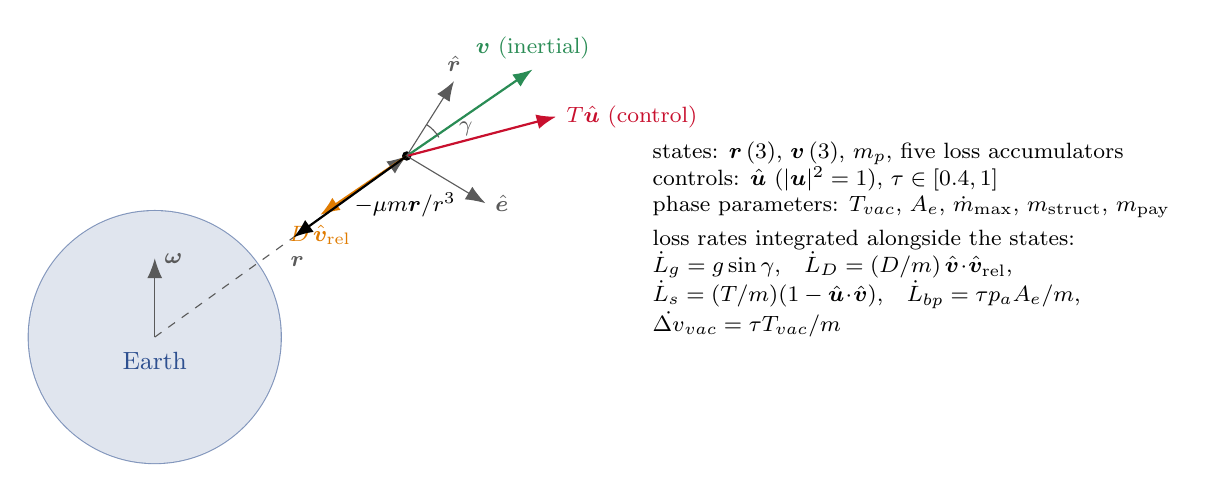
\begin{tikzpicture}[scale=1.0, font=\small, >={Latex[length=2.5mm]}]
  \draw[sfblue!60, thick] (0,0) circle (1.6);
  \fill[sfblue!15] (0,0) circle (1.6);
  \node[sfblue] at (0,-0.3) {Earth};
  \draw[->, sfgrey] (0,0) -- (0,1.0) node[right, font=\footnotesize] {$\bm\omega$};
  \coordinate (P) at (3.2,2.3);
  \draw[->, dashed, sfgrey] (0,0) -- (P) node[midway, below right, font=\footnotesize] {$\bm r$};
  \fill[black] (P) circle (0.06);
  \draw[->, thick, sfgreen] (P) -- ++(1.6,1.1) node[above, font=\footnotesize] {$\bm v$ (inertial)};
  \draw[->, thick, sfred] (P) -- ++(1.9,0.5) node[right, font=\footnotesize] {$T\hat{\bm u}$ (control)};
  \draw[->, thick, sforange] (P) -- ++(-1.1,-0.75) node[below, font=\footnotesize] {$D\,\hat{\bm v}_{\mathrm{rel}}$};
  \draw[->, thick, black] (P) -- ($(P)!0.45!(0,0)$) node[pos=0.6, right=2pt, font=\footnotesize] {$-\mu m\bm r/r^3$};
  \draw[->, sfgrey, thin] (P) -- ++(0.6,0.95) node[above, font=\footnotesize] {$\hat{\bm r}$};
  \draw[->, sfgrey, thin] (P) -- ++(1.0,-0.6) node[right, font=\footnotesize] {$\hat{\bm e}$};
  \draw[sfgrey, thin] ($(P)+(0.25,0.4)$) arc (58:30:0.47); \node[font=\footnotesize, sfgrey] at ($(P)+(0.75,0.35)$) {$\gamma$};
  \node[align=left, font=\footnotesize, anchor=north west] at (6.2,2.6) {
    states: $\bm r\,(3)$, $\bm v\,(3)$, $m_p$, five loss accumulators\\
    controls: $\hat{\bm u}$ ($|\bm u|^2=1$), $\tau\in[0.4,1]$\\
    phase parameters: $T_{vac}$, $A_e$, $\dot m_{\max}$, $m_{\mathrm{struct}}$, $m_{\mathrm{pay}}$\\[3pt]
    loss rates integrated alongside the states:\\
    $\dot L_{g} = g\sin\gamma$,\quad $\dot L_{D} = (D/m)\,\hat{\bm v}\!\cdot\!\hat{\bm v}_{\mathrm{rel}}$,\\
    $\dot L_{s} = (T/m)(1-\hat{\bm u}\!\cdot\!\hat{\bm v})$,\quad $\dot L_{bp} = \tau p_a A_e/m$,\\
    $\dot{\dv}_{vac} = \tau T_{vac}/m$
  };
\end{tikzpicture}
\caption{Forces on the point mass and the quantities carried as states. The loss rates are the terms of
$d|\bm v|/dt = (T/m)\cos\alpha_T - D/m - g\sin\gamma$, so that
$\dv_{vac} = (|\bm v_f|-|\bm v_0|) + L_g + L_D + L_s + L_{bp}$ holds identically --- slide~28 closed numerically.}
\label{fig:forces}
\end{figure}

\subsection{Environment and engine models}
The US Standard Atmosphere 1976 is implemented as a table (analytic layers to 86~km, published values above) and
evaluated as a log-linear interpolant, which keeps $\rho(h)$ and $p_a(h)$ smooth and differentiable to orbit
(Figure~\ref{fig:atm}). It reproduces the notebook's \texttt{ambiance} values to within 0.1\,\% below 81~km.

An engine is specified by one anchor pair ($T_{vac}$, $I_{sp,vac}$) and an exit area; mass flow follows from
$\dot m_{\max} = T_{vac}/(I_{sp,vac}\,g_0)$ and the sea-level thrust and $I_{sp}$ from the back-pressure term
(Figure~\ref{fig:engine}). This matters because published Raptor figures are mutually inconsistent --- Raptor~2's
230~tf~SL / 327~s~SL / 347~s~vac triple \emph{is} consistent with a 1.3~m exit ($p_aA_e = 134$~kN), whereas the
often-quoted 258~tf vacuum thrust would require a 1.86~m exit --- and a lookup table of mixed sources produces an
unphysical engine. In the co-design milestone this block becomes an OpenMDAO group that produces
$(T_{vac}, A_e, \dot m)$ from chamber pressure, expansion ratio and mixture ratio through $c^*$ and $C_F$.

\begin{figure}[h]\centering
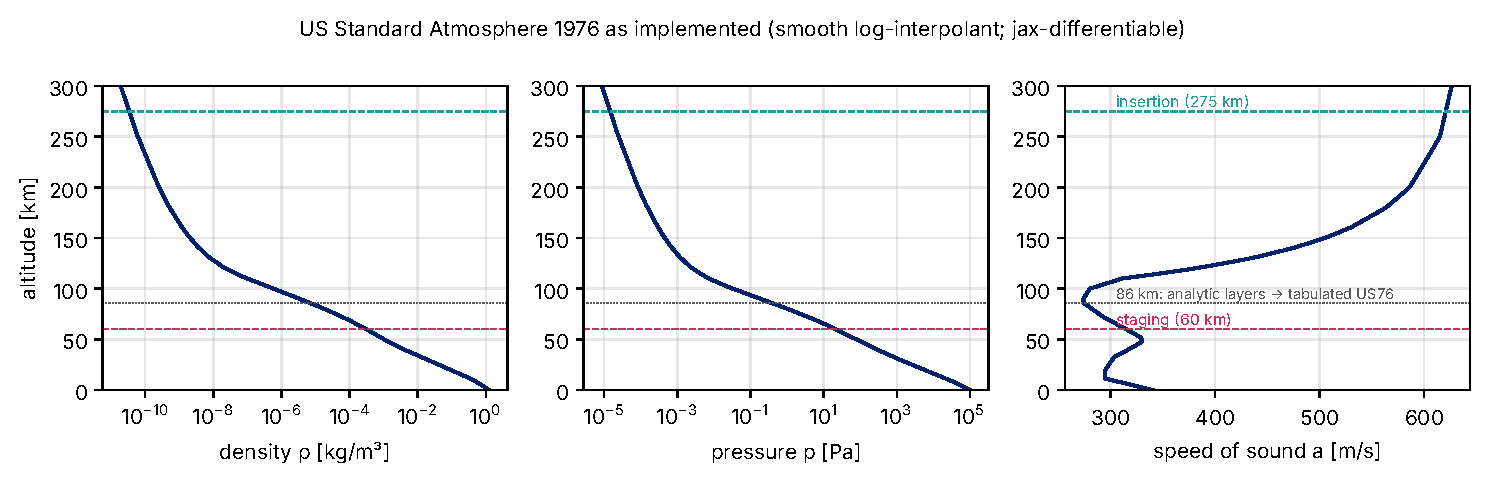
\includegraphics[width=\textwidth]{fig_atmosphere}
\caption{US76 atmosphere as implemented. Dashed lines mark the optimized staging altitude and the target orbit.}
\label{fig:atm}
\end{figure}
\begin{figure}[h]\centering
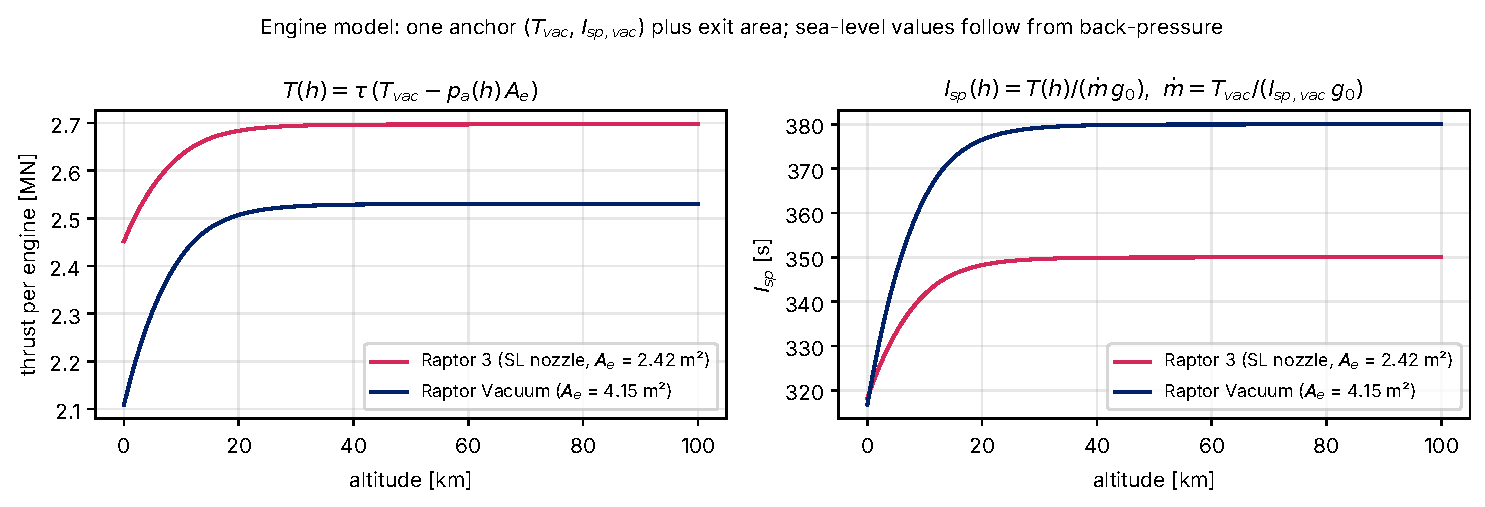
\includegraphics[width=\textwidth]{fig_engine_model}
\caption{Engine model for the two Raptor variants of the Starship deck. Sea-level thrust and $I_{sp}$ are outputs, not inputs.}
\label{fig:engine}
\end{figure}

\section{Optimal-control formulation and numerical method}
\label{sec:method}

\subsection{The problem being solved}
Table~\ref{tab:formulation} lists the problem. Payload is a trajectory-level parameter shared by all phases
and is the design variable the optimizer maximizes; the phase durations are free; the terminal set is a circular
orbit of given altitude with free (or fixed) inclination.

\begin{table}[h]\centering\small
\caption{Optimal-control problem solved for the fixed-vehicle mode.}
\label{tab:formulation}
\begin{tabular}{lp{11.5cm}}
\toprule
Maximize & $m_{\mathrm{pay}}$ (alternatives: minimize propellant used, minimize time) \\
over & $\hat{\bm u}(t)$, $\tau(t)$ in each burn phase; phase durations; $m_{\mathrm{pay}}$ \\
subject to & dynamics of Section~\ref{sec:model} in every phase (collocation defects) \\
 & $|\bm u|^2 = 1$, \; $\tau_{\min}\le\tau\le1$, \; $h\ge0$, \; $q\le q_{\max}$, \; $T/m\le a_{\max}$ (path) \\
 & continuity of $t$, $\bm r$, $\bm v$ and the loss states between phases (linkage) \\
 & $m_p$ fixed to the stage load when a stage ignites; $m_p(t_f) \ge m_{\mathrm{reserve}}$ at burnout (boundary) \\
 & $h(t_f) = h_{\mathrm{target}}$, \; $\gamma(t_f) = 0$, \; $|\bm v(t_f)| = \sqrt{\mu/(R_E+h_{\mathrm{target}})}$ [, $i(t_f) = i_{\mathrm{target}}$] \\
Initial state & $\bm r_0$ at the launch site, $\bm v_0 = \bm\omega\times\bm r_0$, loss states zero; first 10~s vertical at full thrust \\
\bottomrule
\end{tabular}
\end{table}

\subsection{Phases and staging}
Each stage burn is a Dymos phase with its \emph{own} propellant state; the total mass is assembled inside the
ODE from phase parameters (Figure~\ref{fig:phases}). Position, velocity, time and the loss accumulators are linked
between phases; propellant is not, so the mass drop at staging needs no linkage offset and the stage dry masses
can later become design variables without touching the linkages. Return-propellant reserves enter as lower
bounds on the propellant remaining at burnout.

\begin{figure}[h]\centering
\resizebox{\textwidth}{!}{%
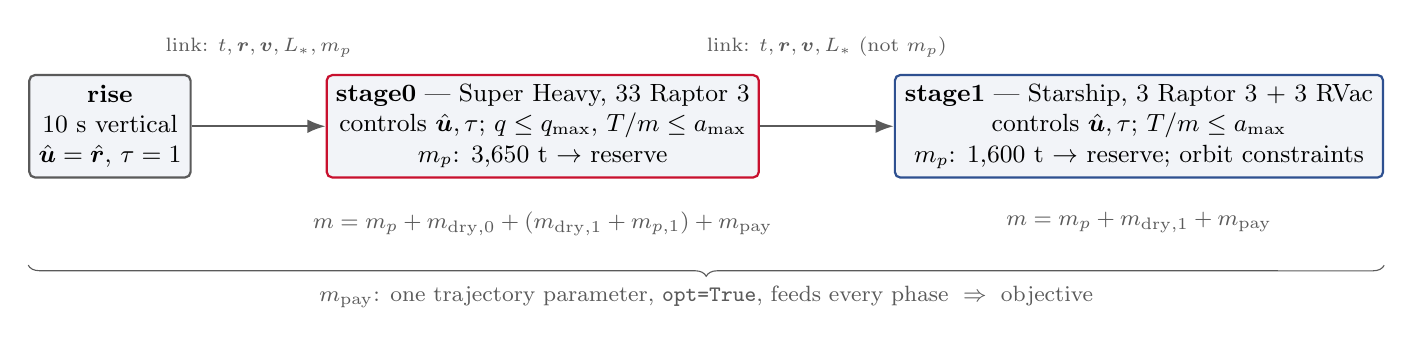
\begin{tikzpicture}[font=\small, >={Latex[length=2.3mm]},
  ph/.style={draw, thick, rounded corners=2pt, minimum height=13mm, align=center, fill=sflight}]
  \node[ph, draw=sfgrey, minimum width=17mm] (rise) {\textbf{rise}\\10~s vertical\\$\hat{\bm u}=\hat{\bm r}$, $\tau=1$};
  \node[ph, draw=sfred, minimum width=50mm, right=17mm of rise] (b) {\textbf{stage0} --- Super Heavy, 33 Raptor~3\\controls $\hat{\bm u},\tau$; $q\le q_{\max}$, $T/m\le a_{\max}$\\$m_p$: 3,650 t $\to$ reserve};
  \node[ph, draw=sfblue, minimum width=62mm, right=17mm of b] (s) {\textbf{stage1} --- Starship, 3 Raptor~3 + 3 RVac\\controls $\hat{\bm u},\tau$; $T/m\le a_{\max}$\\$m_p$: 1,600 t $\to$ reserve; orbit constraints};
  \draw[->, sfgrey, thick] (rise) -- node[above=7.5mm, font=\scriptsize]{link: $t,\bm r,\bm v,L_\ast,m_p$} (b);
  \draw[->, sfgrey, thick] (b) -- node[above=7.5mm, font=\scriptsize]{link: $t,\bm r,\bm v,L_\ast$ (not $m_p$)} (s);
  \node[below=3mm of b, font=\footnotesize, align=center, sfgrey] {$m = m_p + m_{\mathrm{dry,0}} + (m_{\mathrm{dry,1}}+m_{p,1}) + m_{\mathrm{pay}}$};
  \node[below=3mm of s, font=\footnotesize, align=center, sfgrey] {$m = m_p + m_{\mathrm{dry,1}} + m_{\mathrm{pay}}$};
  \draw[decorate, decoration={brace, amplitude=4pt, mirror}, sfgrey] ($(rise.south west)+(0,-11mm)$) -- ($(s.south east)+(0,-11mm)$) node[midway, below=4pt, font=\footnotesize] {$m_{\mathrm{pay}}$: one trajectory parameter, \texttt{opt=True}, feeds every phase $\;\Rightarrow\;$ objective};
\end{tikzpicture}}
\caption{Phase structure. Hot staging is instantaneous in 3-DOF; the booster's reserve and the ship's landing propellant are inputs (not flown).}
\label{fig:phases}
\end{figure}

\subsection{Direct collocation}
Each phase is discretized with the Legendre--Gauss--Radau pseudospectral transcription (Figure~\ref{fig:colloc}):
the states are polynomials of degree 3 on each of 16 segments, the controls are polynomials on the same segments,
and the dynamics are enforced as \emph{defect constraints} at the collocation nodes. The result is a large, sparse
nonlinear program (1,288 variables and 1,474 constraints for the two-stage case at 12 segments) rather than a
sequence of simulations: the optimizer sees all of the trajectory at once, infeasible intermediate iterates are
allowed, and the Jacobian is exact. Three implementation facts decided whether this converged:
\begin{enumerate}
  \item \textbf{Derivatives.} The ODE is an OpenMDAO \texttt{JaxExplicitComponent}: partials come from automatic
        differentiation (checked against finite differences to $10^{-10}$). The node-diagonal sparsity of the partials
        must be \emph{declared}, because OpenMDAO builds the total-Jacobian sparsity from declared patterns; undeclared,
        the coloring needed 504 colors for 843 variables, declared it needs 43.
  \item \textbf{Smooth outputs.} Flight-path angle, angle of attack and inclination are computed with $\arctan2$;
        the $\arcsin/\arccos$ forms have infinite slope exactly where a gravity-turn guess sits (thrust along velocity)
        and produced a dual infeasibility of $10^9$. The insertion constraint is $\gamma = 0$ rather than
        $\bm r\cdot\bm v = 0$, whose natural scale ($10^{10}\unit{m^2/s}$) defeats the scaling.
  \item \textbf{Optimizer.} IPOPT (through pyoptsparse/cyipopt, limited-memory Hessian, MUMPS). SciPy's SLSQP fails even
        Dymos's own single-stage benchmark; IPOPT solves it in 27 iterations.
\end{enumerate}

\begin{figure}[h]\centering
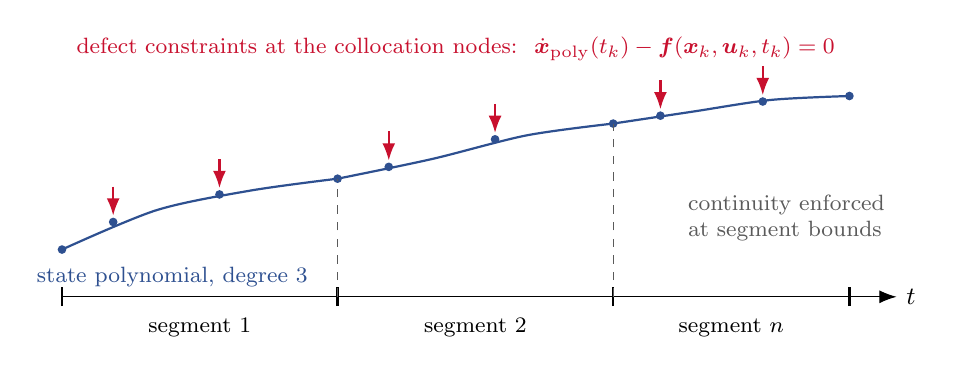
\begin{tikzpicture}[font=\small, >={Latex[length=2.2mm]}, xscale=1.0]
  \draw[->] (0,0) -- (10.6,0) node[right] {$t$};
  \foreach \x in {0,3.5,7,10} \draw[thick] (\x,-0.12) -- (\x,0.12);
  \node[below, font=\footnotesize] at (1.75,-0.15) {segment 1};
  \node[below, font=\footnotesize] at (5.25,-0.15) {segment 2};
  \node[below, font=\footnotesize] at (8.5,-0.15) {segment $n$};
  \draw[sfblue, thick] plot[smooth] coordinates {(0,0.6) (1.2,1.1) (2.4,1.35) (3.5,1.5)};
  \draw[sfblue, thick] plot[smooth] coordinates {(3.5,1.5) (4.7,1.75) (5.9,2.05) (7,2.2)};
  \draw[sfblue, thick] plot[smooth] coordinates {(7,2.2) (8,2.35) (9,2.5) (10,2.55)};
  \foreach \x/\y in {0/0.6, 0.65/0.95, 2.0/1.3, 3.5/1.5, 4.15/1.65, 5.5/2.0, 7/2.2, 7.6/2.3, 8.9/2.48, 10/2.55}
     \fill[sfblue] (\x,\y) circle (0.055);
  \foreach \x/\y in {0.65/0.95, 2.0/1.3, 4.15/1.65, 5.5/2.0, 7.6/2.3, 8.9/2.48}
     \draw[sfred, ->, thick] (\x,\y+0.45) -- (\x,\y+0.08);
  \node[sfred, font=\footnotesize, align=left] at (5.0,3.15) {defect constraints at the collocation nodes:\; $\dot{\bm x}_{\mathrm{poly}}(t_k) - \bm f(\bm x_k,\bm u_k,t_k) = 0$};
  \node[sfblue, font=\footnotesize] at (1.4,0.25) {state polynomial, degree 3};
  \draw[dashed, sfgrey] (3.5,0) -- (3.5,1.5); \draw[dashed, sfgrey] (7,0) -- (7,2.2);
  \node[font=\footnotesize, sfgrey, align=left] at (9.2,1.0) {continuity enforced\\at segment bounds};
\end{tikzpicture}
\caption{Direct collocation (Radau, order 3). States and controls are discretized on segments; dynamics become algebraic constraints solved simultaneously with the optimization.}
\label{fig:colloc}
\end{figure}

\subsection{Initial guess}
The slide-33 guidance law (vertical rise, pitch kick, thrust along the air-relative velocity) integrated with
\texttt{solve\_ivp} supplies the initial guess; the kick angle is tuned so that the flight-path angle is zero at
burnout. For Starship this gives a trajectory that reaches $\gamma = 0$ at 218~km with 10.1~km/s --- an eccentric
orbit with 2.4~km/s of excess speed --- which the optimizer converts into payload. Cases are warm-started from the
nearest solved case; a cold start of the baseline converges in about 260 IPOPT iterations and a warm-started
sweep case in 20--50.

\section{Example: Starship/Super Heavy Block 3 to \texorpdfstring{$275\unit{km}\times26^\circ$}{275 km x 26 deg}}
\label{sec:example}

\subsection{Inputs}
Table~\ref{tab:inputs} is the deck. Propellant loads and engine numbers are SpaceX's published Block~3 figures;
the dry masses are \emph{not} published and the slide-42 ranges (160--200~t booster, 85--100~t ship) are used as a
baseline and swept. The mission is the course's ``100~t to LEO'' project option from Starbase ($26.0^\circ$N),
275~km circular (the altitude of Flight~14, the first orbital Starship flight, 28~Sep~2026), free inclination
(eastward launch gives $i = 26.0^\circ$), with $q\le35\unit{kPa}$ and $T/m\le4\,g$.

\begin{table}[h]\centering\footnotesize
\caption{Vehicle and mission inputs (\texttt{vehicles/starship\_v3\_baseline.yaml}).}
\label{tab:inputs}
\begin{tabular}{p{3.1cm}p{3.6cm}p{3.6cm}p{4.6cm}}
\toprule
Quantity & Super Heavy & Starship & Source / note \\
\midrule
Propellant load & 3,650 t & 1,600 t & SpaceX Block 3 \\
Dry mass (baseline; swept) & 200 t & 100 t & slide 42 mid-range; not published \\
Engines & 33 $\times$ Raptor 3 & 3 Raptor 3 + 3 RVac & SpaceX \\
Raptor 3 (SL nozzle) & \multicolumn{2}{p{7.4cm}}{250 tf SL / 275 tf vac, $I_{sp,vac}$ 350 s $\Rightarrow$ $A_e$ = 2.42 m$^2$, $I_{sp,SL}$ = 318 s} & SpaceX May 2026 / Aug 2024 \\
Raptor Vacuum & \multicolumn{2}{p{7.4cm}}{258 tf, $I_{sp,vac}$ 380 s, 2.3 m exit diameter} & Week 9 slide 43 \\
Derived stage $T_{vac}$, $\dot m$ & 89.0 MN, 25,930 kg/s & 15.7 MN, 4,394 kg/s & engine model \\
Liftoff $T/W$ (sea level) & 1.46 & 0.89 at ignition (vac) & engine model \\
Throttle range & 0.40--1.00 & 0.40--1.00 & Raptor family \\
Diameter, $C_D$ & \multicolumn{2}{l}{9 m, 0.5 (constant)} & notebook values \\
Reserves (baseline) & 0 & 0 & swept: 292 / 548 t booster, 30 t ship \\
Mission & \multicolumn{3}{p{12cm}}{Starbase 25.997$^\circ$N, 275 km circular, inclination free, $q_{\max}$ = 35 kPa, $a_{\max}$ = 4 $g$, 10 s vertical rise} \\
\bottomrule
\end{tabular}
\end{table}

\subsection{Baseline solution}
Figures~\ref{fig:hist}--\ref{fig:steer} show the converged baseline (16 Radau segments per phase; IPOPT
``solved to acceptable level'', constraint violation $<10^{-7}$). The optimizer finds
\textbf{293.3~t} of payload. The booster throttles to 0.74 between 50 and 75~s to hold $q = 35\unit{kPa}$
(the constraint is active --- Figure~\ref{fig:hist}, right-middle panel), returns to full thrust, and reaches
the 4~$g$ acceleration limit exactly at MECO: $t = 144.7\unit{s}$, $h = 60.4\unit{km}$, $v = 2.61\unit{km/s}$ inertial.
The ship burns 463~s and throttles to its 40\,\% floor for the last 170~s; insertion is at $t = 607.7\unit{s}$
with $h = 275.000\unit{km}$, $\gamma = 5\times10^{-10}$~deg, $|\bm v| = 7{,}740.26\unit{m/s}$, $i = 25.997^\circ$. Both stages
burn to their (zero) reserves. Table~\ref{tab:baseline} summarizes the numbers and the $\dv$ budget.

\begin{figure}[p]\centering
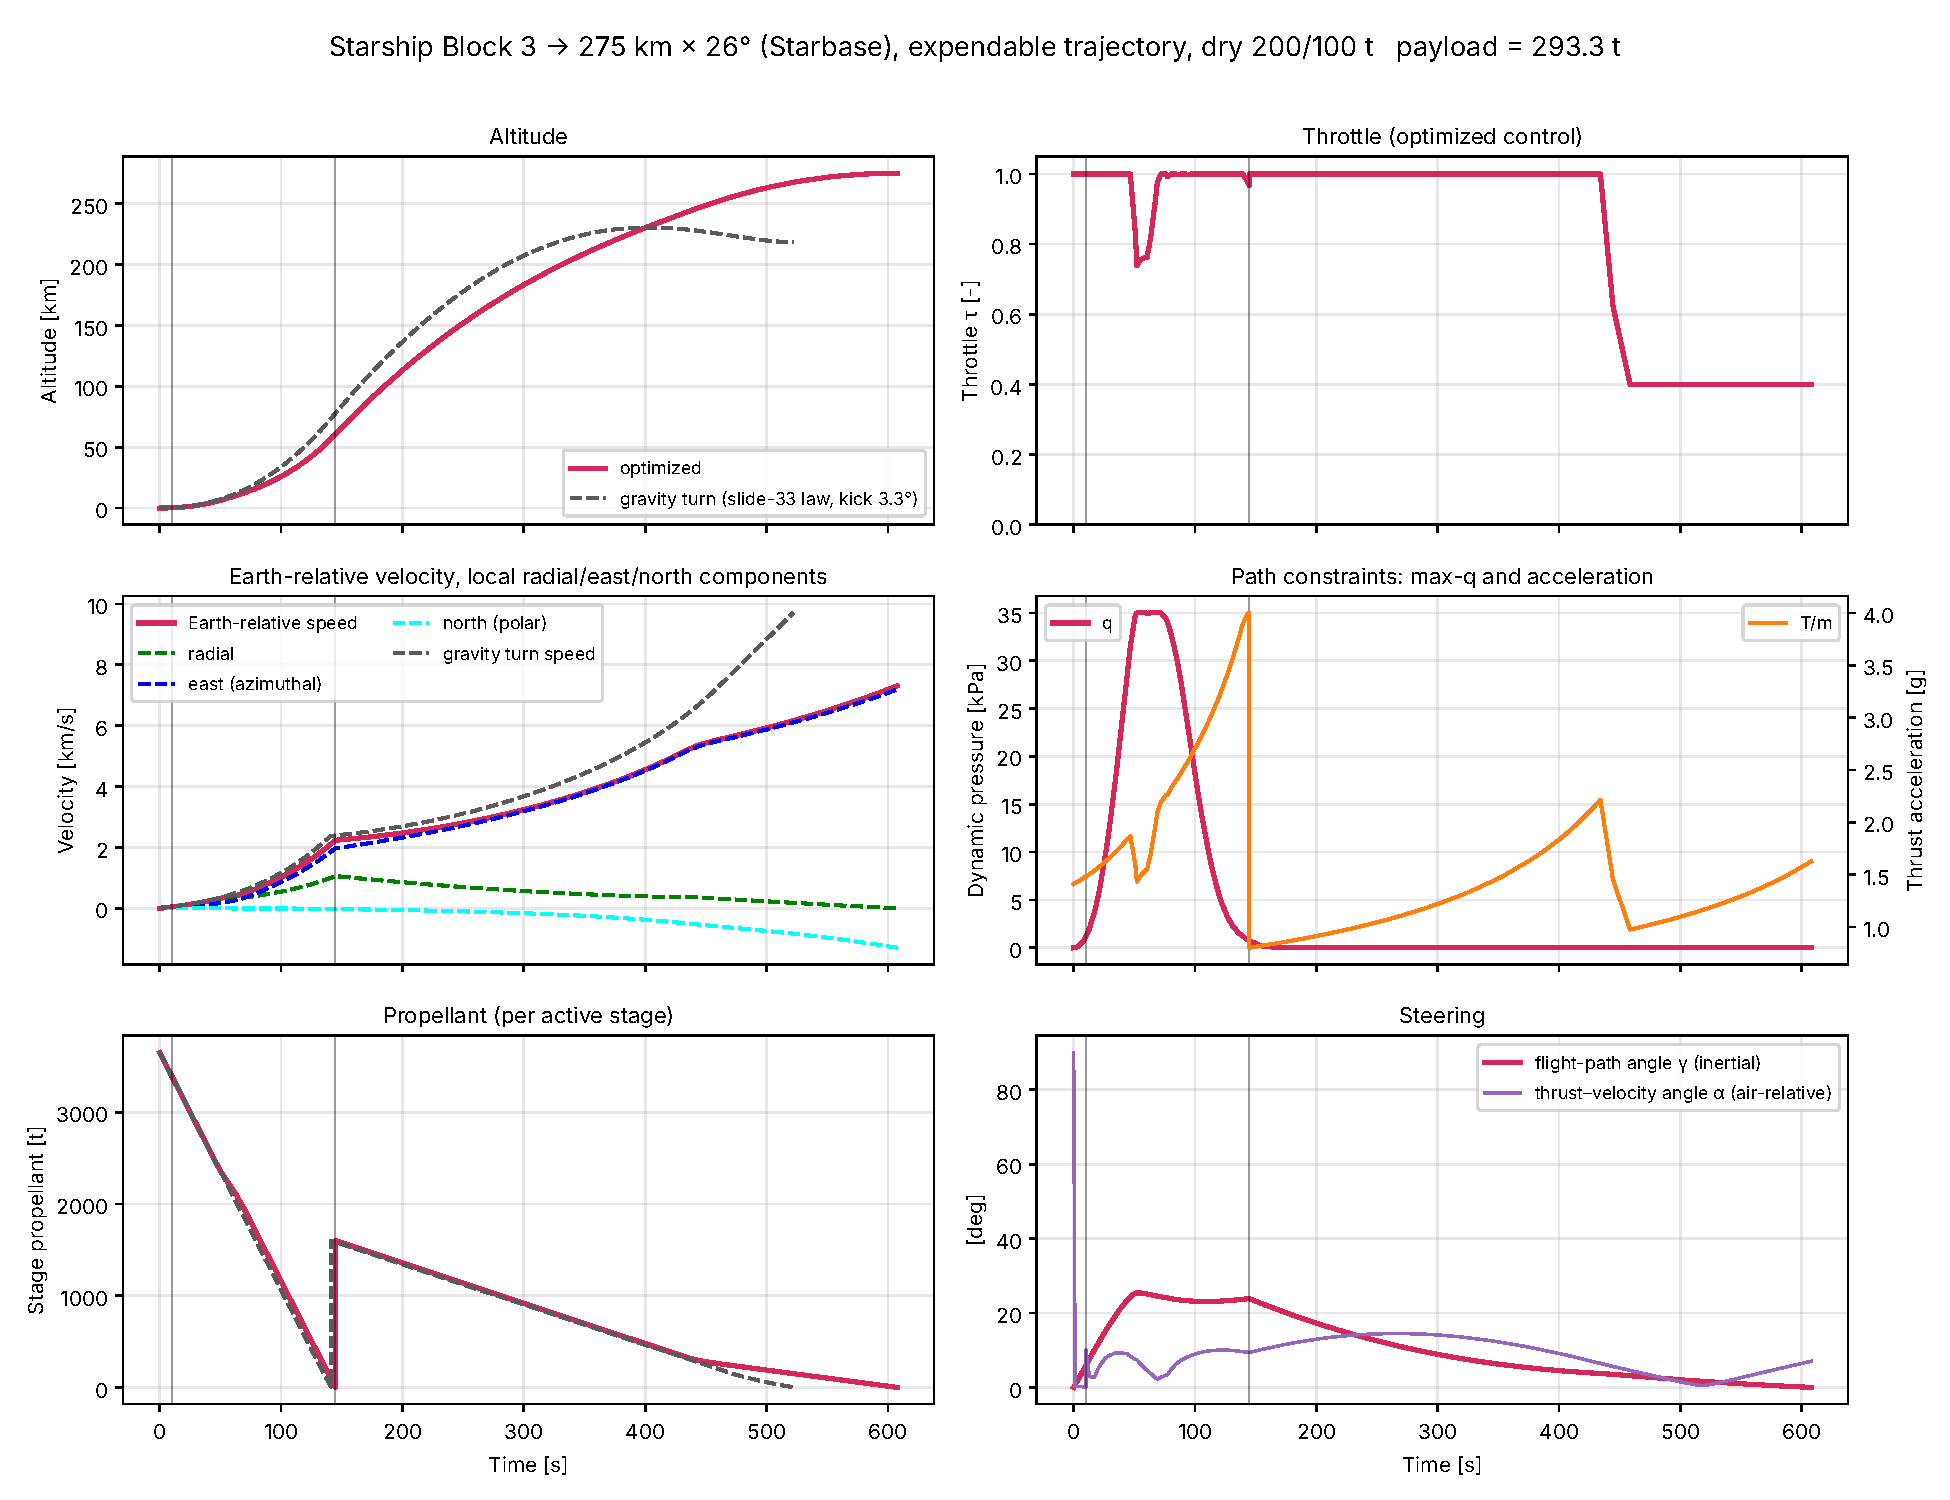
\includegraphics[width=\textwidth]{fig_histories}
\caption{Baseline solution (red) against the slide-33 gravity-turn law applied to the same vehicle (grey dashed).
Left column: the slide-33 layout --- altitude, Earth-relative velocity components, stage propellant. Right column:
throttle, the two active path constraints, flight-path angle and thrust--velocity angle. Vertical lines mark phase boundaries.}
\label{fig:hist}
\end{figure}

\begin{figure}[p]\centering
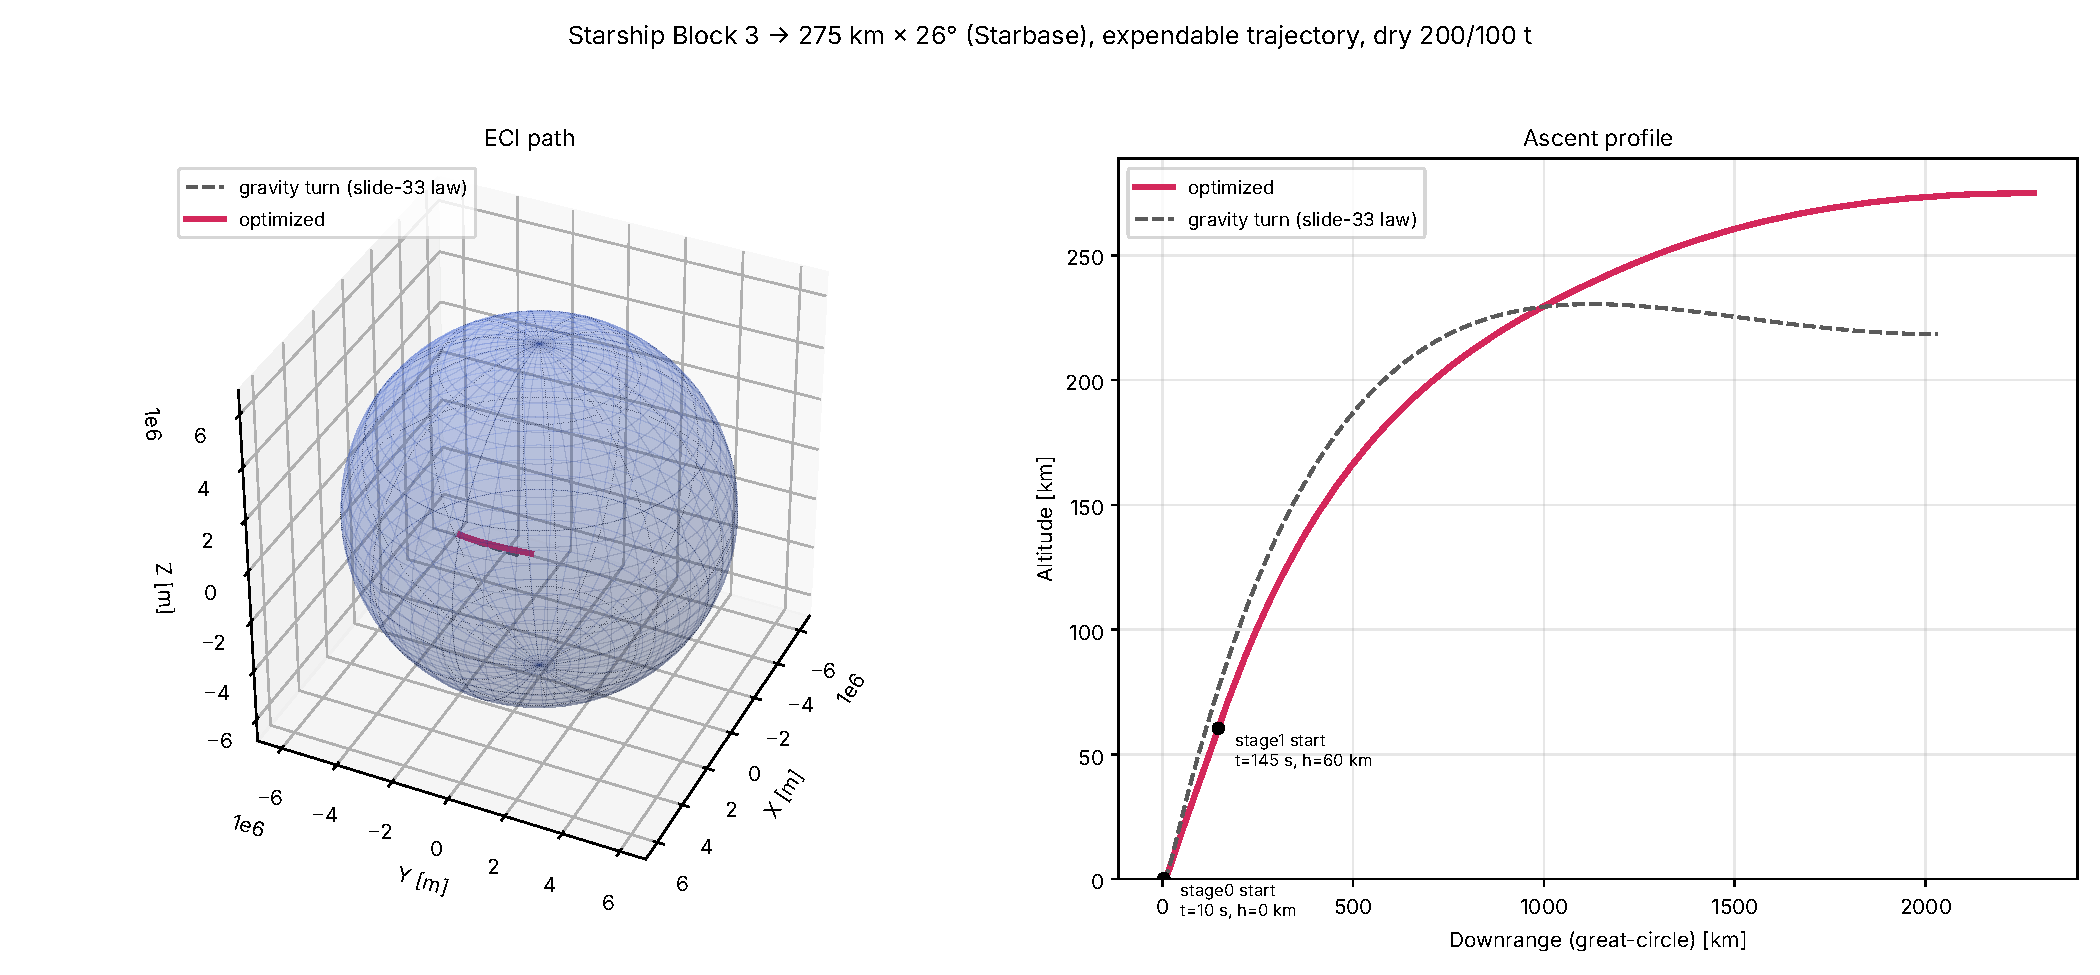
\includegraphics[width=\textwidth]{fig_path3d}
\caption{ECI path on the globe and the ascent profile. The gravity-turn law lofts to 218~km with 10.1~km/s (eccentric orbit); the optimizer inserts into the 275~km circle and carries the difference as payload.}
\label{fig:path}
\end{figure}

\begin{figure}[p]\centering
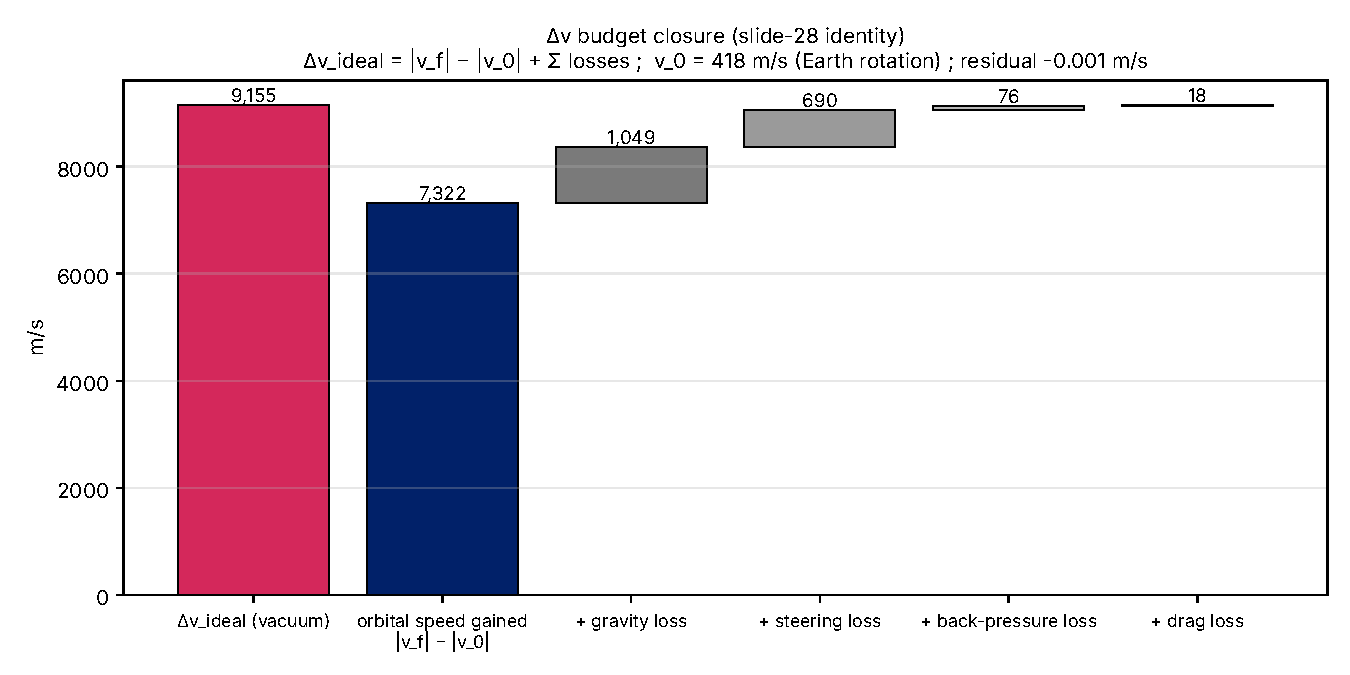
\includegraphics[width=0.9\textwidth]{fig_losses}
\caption{$\dv$ budget closure at the optimum. $\dv_{vac} = 9{,}155 = 7{,}322 + 1{,}049 + 690 + 76 + 18\unit{m/s}$; the residual of the identity is $-0.001\unit{m/s}$. Total losses 1,833~m/s, inside the 1.5--2.0~km/s band of slide~32.}
\label{fig:losses}
\end{figure}

\begin{figure}[p]\centering
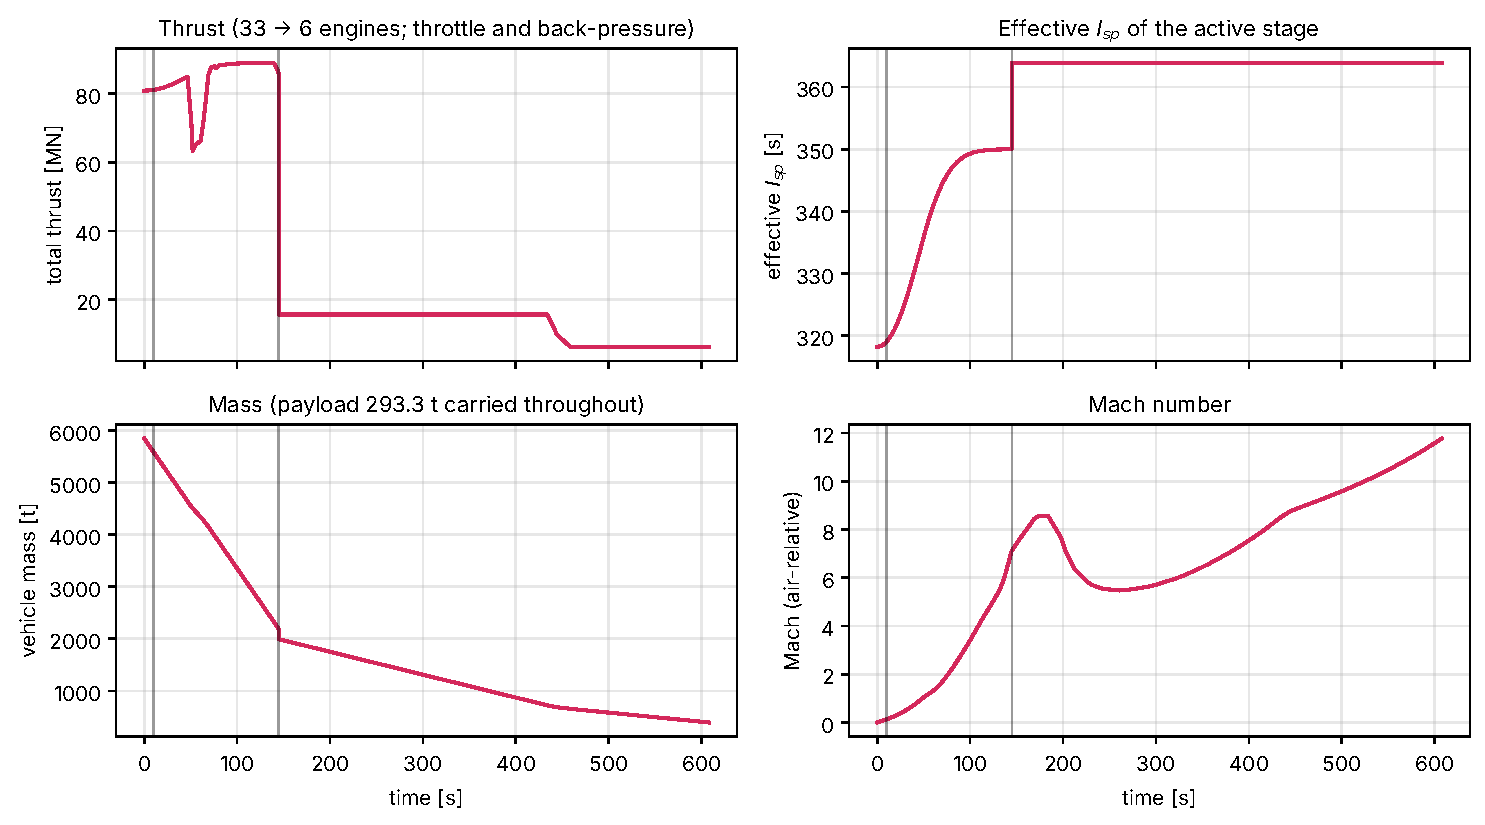
\includegraphics[width=\textwidth]{fig_thrust_isp_mass}
\caption{Thrust, effective $I_{sp}$ of the active stage, vehicle mass and air-relative Mach number. The $I_{sp}$ rise in the first 60~s is the back-pressure term; the step at 145~s is staging onto the Raptor~3/RVac set (thrust-weighted 363.9~s). Mach is shown for completeness only above $\sim$90~km.}
\label{fig:thrust}
\end{figure}

\begin{figure}[p]\centering
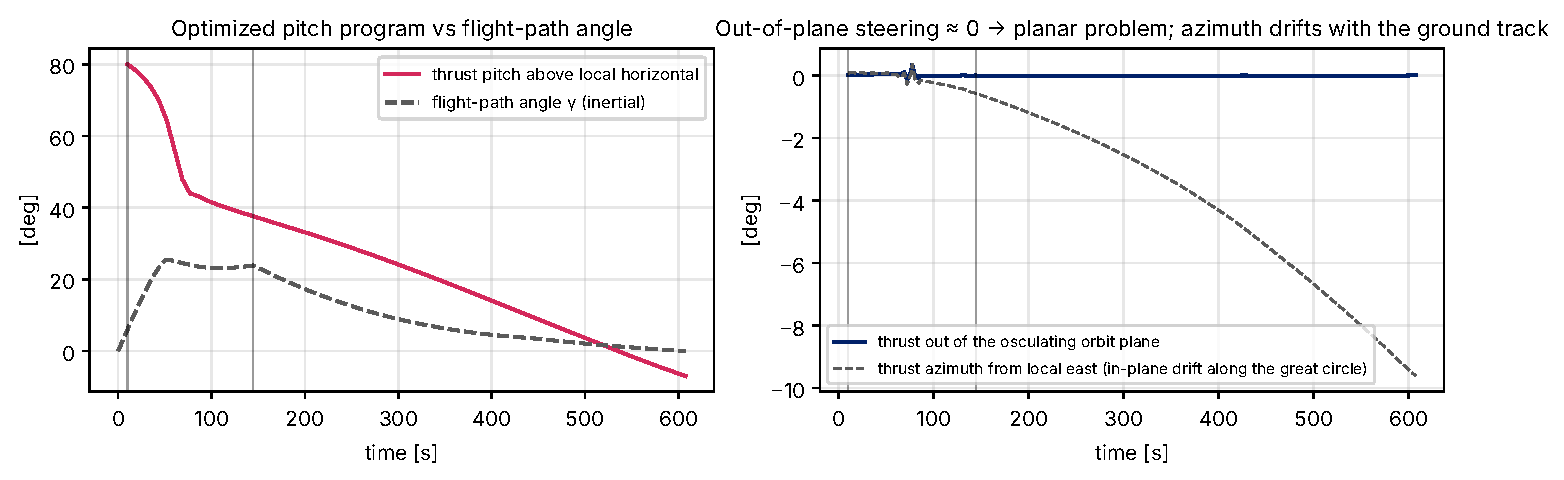
\includegraphics[width=\textwidth]{fig_steering}
\caption{The optimized steering. Left: thrust pitch relative to the local horizontal and flight-path angle. Right: the component of thrust out of the osculating orbit plane is zero to plotting accuracy --- the optimizer discovers that an eastward launch is a planar problem --- while the azimuth measured from local east drifts as the ground track leaves the $26^\circ$N apex of the orbit.}
\label{fig:steer}
\end{figure}

\begin{table}[h]\centering\footnotesize
\caption{Baseline results (dry 200/100~t, no reserves).}
\label{tab:baseline}
\begin{tabular}{>{\raggedright\arraybackslash}p{6.9cm}>{\raggedright\arraybackslash}p{8.6cm}}
\toprule
\multicolumn{2}{l}{\textit{Trajectory}} \\
Payload to $275\unit{km}\times26.0^\circ$ & \textbf{293.3 t} \\
GLOW & 5,843 t \\
Staging (MECO) & 144.7 s, 60.4 km, 2.61 km/s inertial \\
Max-$q$ (constraint active) & 35.0 kPa at 50--75 s, booster throttle down to 0.74 \\
Max $T/m$ (constraint active) & 4.00 $g$ at MECO \\
Ship burn & 463 s; $\tau = 0.40$ for the last 170 s \\
Insertion & 607.7 s; $h$ = 275.000 km, $\gamma = 5\times10^{-10}$ deg, $|\bm v|$ = 7,740.26 m/s, $i = 25.997^\circ$ \\
\midrule
\multicolumn{2}{l}{\textit{$\dv$ budget} (m/s)} \\
$\dv_{vac}$ (both stages, vacuum-referenced) & 9,155 \\
orbital speed gained $|\bm v_f| - |\bm v_0|$ ($|\bm v_0|$ = 418, Earth rotation at 26$^\circ$N) & 7,322 \\
gravity loss $\int g\sin\gamma\,dt$ & 1,049 \\
steering loss $\int (T/m)(1-\cos\alpha_T)\,dt$ & 690 \\
back-pressure loss $\int \tau p_a A_e/m\,dt$ & 76 \\
drag loss $\int D/m\,dt$ & 18 \\
identity residual & $-0.001$ \\
\bottomrule
\end{tabular}
\end{table}

\subsection{What the payload depends on}
Seven cases were run from the baseline by overriding deck values on the command line (Table~\ref{tab:sweep},
Figure~\ref{fig:sweep}). Three results are worth stating in class:
\begin{enumerate}
  \item \textbf{Ship dry mass trades 1:1 with payload.} The four no-reserve cases are reproduced to 0.07~t by
        $m_{\mathrm{pay}} = 425.8 - 0.161\,m_{\mathrm{dry,booster}} - 1.001\,m_{\mathrm{dry,ship}}$ [t]
        (Figure~\ref{fig:sens}, left): a kilogram on the ship is a kilogram of payload, a kilogram on the booster costs
        160~g.
  \item \textbf{Return-propellant reserves are the largest lever.} Holding back 8\,\% of the booster propellant (292~t)
        plus 30~t in the ship costs 89~t of payload; 15\,\% costs 131~t. The optimizer moves the staging point by itself
        --- from 145~s/60~km/2.61~km/s to 133~s/53~km/2.29~km/s at 8\,\% and 123~s/47~km/2.00~km/s at 15\,\%
        (Figure~\ref{fig:reserve}) --- which is the mechanism behind the ``stage low for reusability'' rule.
  \item \textbf{The gap to the published 100~t is attributable.} Even the pessimistic corner (dry 250/120~t plus
        8\,\% reserve) gives 178~t. What remains is outside this model: the actual ship dry mass with heat shield and
        flaps (likely well above 120~t), boost-back propellant that grows with staging speed and must deliver a
        specific return trajectory rather than an 8\,\% allowance, engine performance margins and operational
        margins. The tool's contribution is to make the gap a list of named quantities with known sensitivities.
\end{enumerate}

\begin{table}[h]\centering\small
\caption{Sweep results. All cases converged (IPOPT acceptable level, constraint violation $\le10^{-7}$); iterations are for the warm-started final chunk.}
\label{tab:sweep}
\footnotesize
\setlength{\tabcolsep}{4pt}
\begin{tabular}{>{\raggedright\arraybackslash}p{4.9cm}rrrrrr}
\toprule
Case & Payload [t] & Stage $t$ [s] & $h$ [km] & $v$ [km/s] & $L_g$ [m/s] & $L_s$ [m/s] \\
\midrule
dry 160/85 t (slide-42 low), no reserves & 314.9 & 144.6 & 61.1 & 2.65 & 1,045 & 680 \\
\textbf{baseline: dry 200/100 t, no reserves} & \textbf{293.3} & 144.7 & 60.4 & 2.61 & 1,049 & 690 \\
dry 250/120 t, no reserves & 265.3 & 144.4 & 59.8 & 2.57 & 1,056 & 702 \\
ship dry 150 t (booster 200 t), no reserves & 243.3 & 144.7 & 60.4 & 2.61 & 1,049 & 690 \\
reserves: booster 292 t (8\,\%), ship 30 t & 204.5 & 133.4 & 53.0 & 2.29 & 1,083 & 716 \\
dry 250/120 t + reserves 292/30 t & 178.4 & 133.1 & 52.4 & 2.25 & 1,090 & 727 \\
reserves: booster 548 t (15\,\%), ship 30 t & 162.7 & 123.3 & 46.5 & 2.00 & 1,126 & 753 \\
\bottomrule
\end{tabular}
\end{table}

\begin{figure}[p]\centering
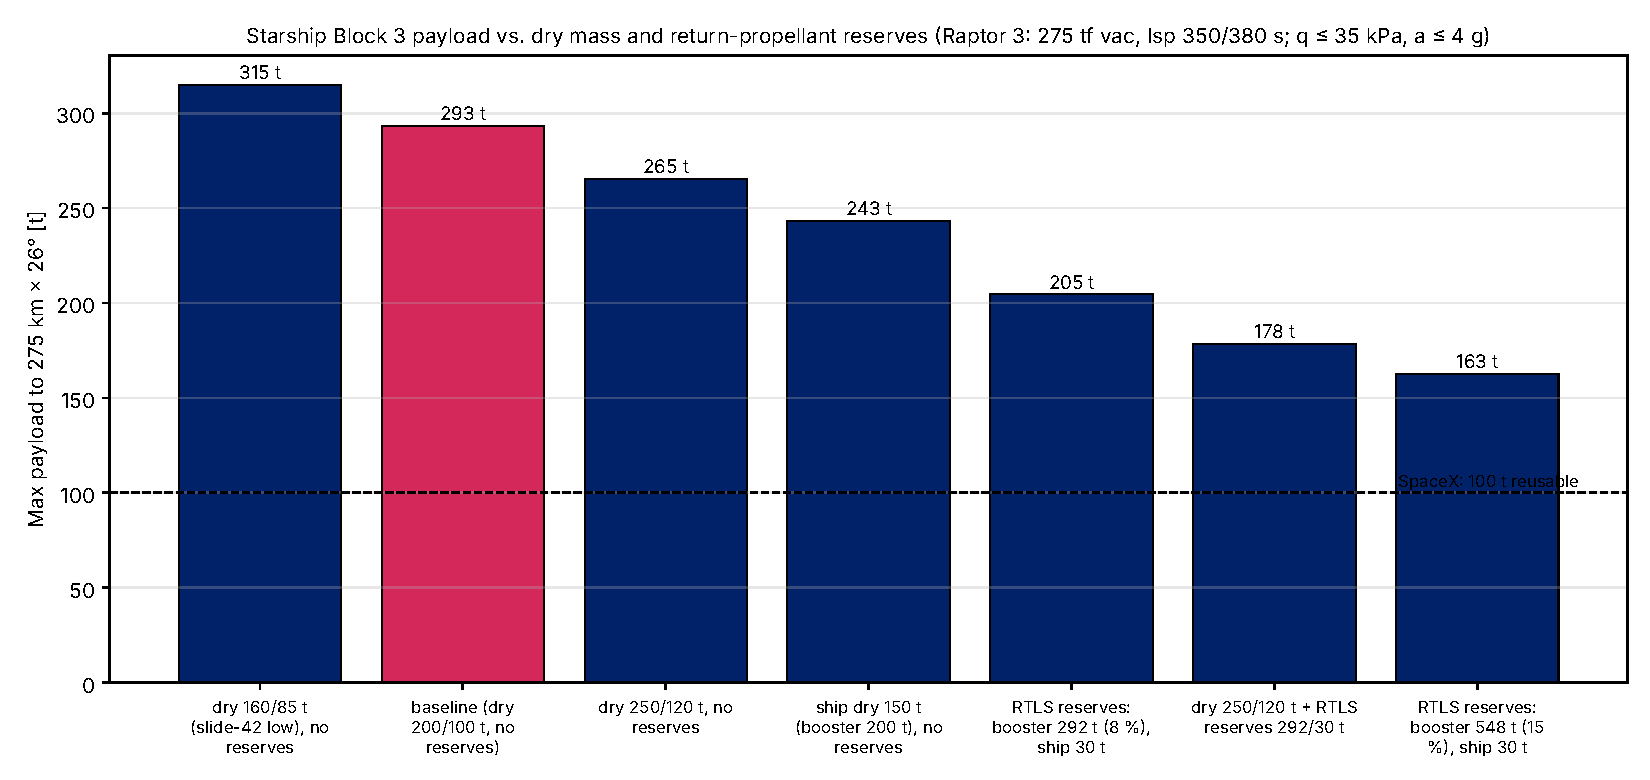
\includegraphics[width=\textwidth]{fig_sweep}
\caption{Maximum payload across the sweep. The dashed line is SpaceX's published reusable figure.}
\label{fig:sweep}
\end{figure}
\begin{figure}[p]\centering
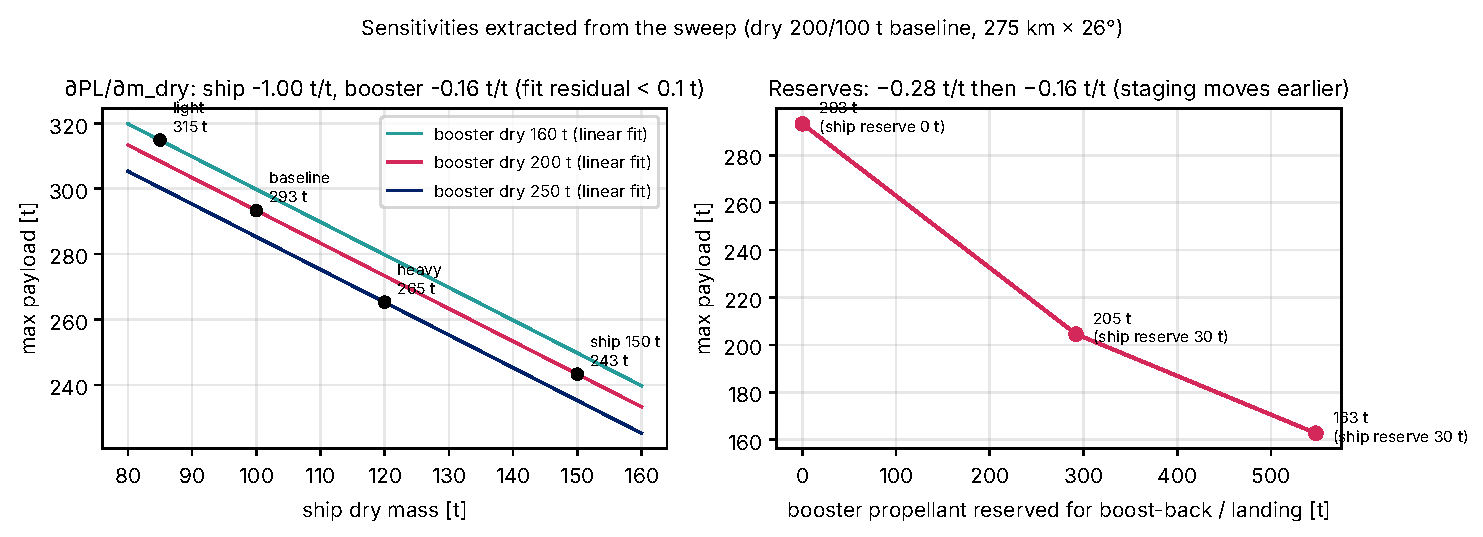
\includegraphics[width=\textwidth]{fig_sensitivity}
\caption{Sensitivities extracted from the sweep. Left: a linear model in the two dry masses reproduces the four no-reserve cases to 0.07~t. Right: payload against booster propellant held back for return; the slope flattens because the optimizer re-stages earlier.}
\label{fig:sens}
\end{figure}
\begin{figure}[htbp]\centering
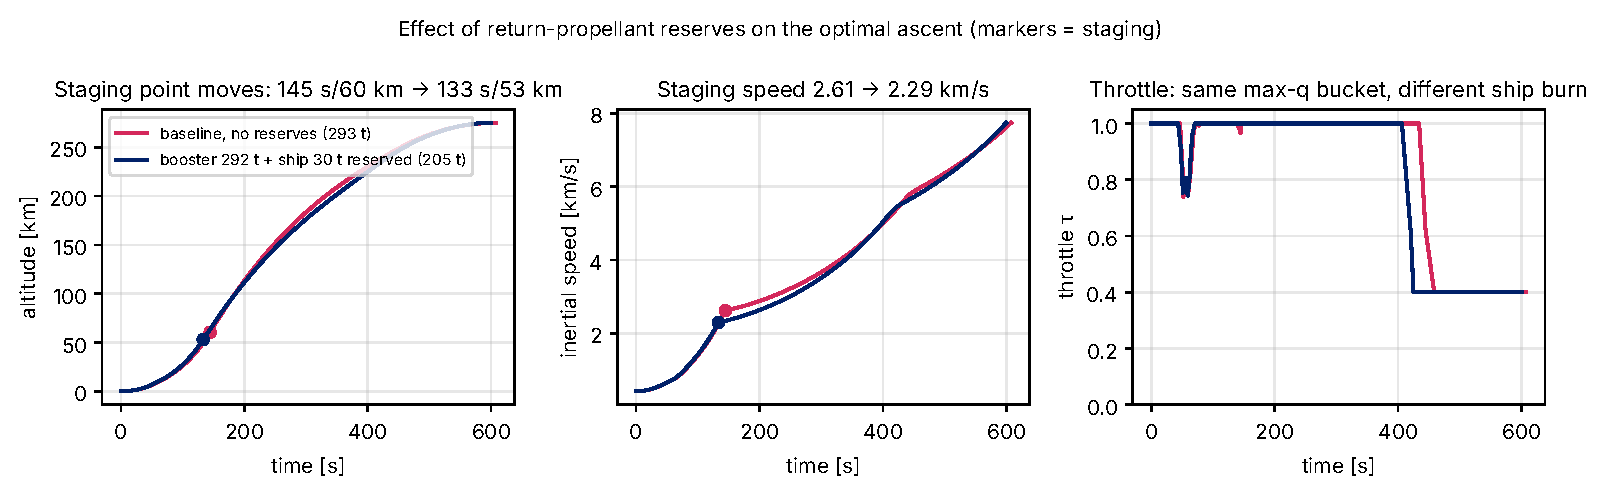
\includegraphics[width=\textwidth]{fig_reserve_compare}
\caption{Baseline versus the 8\,\%-reserve case. The max-$q$ throttle bucket is unchanged; the staging point moves earlier and lower and the ship carries more of the $\dv$.}
\label{fig:reserve}
\end{figure}

\section{Verification}
\label{sec:verification}
Table~\ref{tab:verif} lists what was checked. The explicit re-integration (Figure~\ref{fig:verif}) restarts from the
collocation state at each phase boundary and drifts by 211~m and 4.5~m/s by insertion; the drift originates at the
throttle transition at 440~s, where the piecewise-polynomial control is least accurate, and halves from 12 to 16
segments. Grid refinement at that transition is the obvious next step and does not change the payload at the
0.04\,\% level.

\begin{table}[h]\centering\small
\caption{Verification performed on 9~Nov~2026.}
\label{tab:verif}
\begin{tabular}{p{6.2cm}p{9.3cm}}
\toprule
Check & Result \\
\midrule
Benchmark: Dymos SSTO (Longuski Titan~II min-time) with IPOPT & $t_f = 143.77$~s in 27 iterations (documented $\approx 143$~s); SciPy SLSQP failed in 3,000 iterations \\
Explicit re-integration of optimized controls (\texttt{simulate}) & 16 segments: $+211$~m, $+4.5$~m/s, $0.0002^\circ$ at insertion; 12 segments: $+322$~m, $+8.8$~m/s \\
Grid independence & 293.20~t (12 segments) vs 293.31~t (16 segments) \\
Loss identity $\dv_{vac} = \Delta|\bm v| + \sum L$ & residual $\le 0.004$~m/s in all seven cases \\
ODE partials (jax) vs finite differences & agree to $\sim10^{-10}$ \\
US76 table vs the notebook's \texttt{ambiance} & $<0.1\,\%$ in $\rho$, $p$ below 81~km \\
Rocket-equation consistency & with the optimizer's $\dv_{vac}$ the hand calculation returns the optimizer's payload (Table~\ref{tab:tsiolkovsky}) \\
Flight data (IFT-3 public timeline: staging 72~km, T+170~s, return-to-site profile) & 53~km/133~s with 8\,\% reserve, 47~km/123~s with 15\,\% --- same regime; lower because reserves are allowances, not a flown return \\
\bottomrule
\end{tabular}
\end{table}

\begin{figure}[htbp]\centering
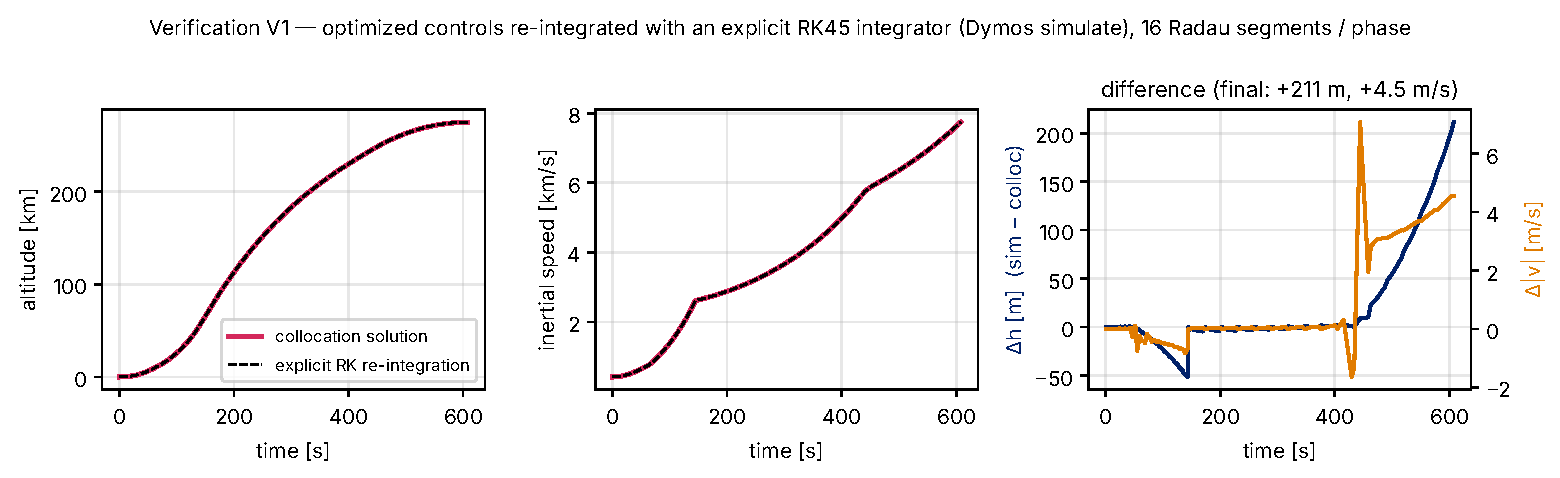
\includegraphics[width=\textwidth]{fig_verification}
\caption{Collocation solution versus explicit RK45 re-integration of the optimized controls. Right: the difference, which starts at the 440~s throttle transition.}
\label{fig:verif}
\end{figure}

\FloatBarrier
\section{Limitations and next steps}
\label{sec:next}
\begin{itemize}
  \item \textbf{Aerodynamics.} $C_D$ is constant; a Mach-dependent table is the first refinement (affects drag loss and the max-$q$ bucket, both small here).
  \item \textbf{Gravity, winds.} Point-mass spherical Earth, no $J_2$, no winds, no 6-DOF.
  \item \textbf{Reusability.} Reserves are inputs; boost-back and landing are not simulated, so the reserve--staging-speed coupling that drives real return-to-site designs is not closed.
  \item \textbf{Solution structure.} The ship's final 40\,\%-throttle arc is what IPOPT returned on this grid; it should be re-checked with grid refinement and a different initial guess before drawing conclusions from it.
  \item \textbf{Unphysical vehicles.} The notebook's own ``Falcon-9-like'' single stage ($T/W = 3.75$, 95\,\% propellant fraction) did not converge as a max-payload problem; a feasibility run reached 250~km with $\approx 0$ payload and 79~$g$ at burnout. It is not a useful test case.
  \item \textbf{Co-design (milestone 2--3).} Engine model from $(p_c, \varepsilon, O/F)$ via $c^*$ and $C_F$, stage mass model, and the FFSC-cycle/turbopump models as OpenMDAO components in the same problem --- the reason Dymos was chosen. In-space mission module (Hohmann/Lambert, $C_3$, aerocapture) for the Mars, Moon and Titan project missions.
\end{itemize}

\section{Using the tool}
\begin{lstlisting}
conda env create -f environment.yml && conda activate ascentopt
python scripts/run_case.py --vehicle vehicles/starship_v3_baseline.yaml --out runs/starship \
    --h-target 275e3 --lat 25.997 --q-max 35e3 --a-max 39.2266 --segments 16 --max-iter 400 --simulate
python scripts/run_case.py ... --out runs/heavy --warm-from runs/starship/*_out/dymos_solution.db \
    --set stage0.dry_mass=250e3 --set stage1.dry_mass=120e3
python scripts/make_figures.py runs/starship --out results/figs
bash reproduce_demo.sh      # baseline + six-case sweep + figures
\end{lstlisting}
The environment is conda-forge (OpenMDAO 3.41, pyoptsparse 2.17, cyipopt 1.7/Ipopt 3.14, jax 0.7) plus
dymos 1.16 from PyPI. \texttt{cyipopt} must be listed explicitly or the IPOPT driver fails to import. Results
land in \texttt{result.json} next to the Dymos record \texttt{dymos\_solution.db}; \texttt{--restart} resumes a case
and \texttt{--warm-from} starts a new case from another case's record with the new deck re-applied.

\section*{Sources}
\begin{itemize}\small
  \item SpaceX Starship and Raptor data as compiled on Wikipedia (Block~2/3 propellant loads, engine counts, Raptor~3 250/275~tf and 350~s, Flight~14 orbit) and in the New Space Economy review of Starship V3 (April 2026); Week~9 slides 42--43 for the Raptor/RVac figures used there.
  \item Dymos documentation: SSTO Earth-launch example (Longuski Titan~II benchmark), Trajectory API; OpenMDAO \texttt{JaxExplicitComponent}.
  \item IFT-3 timeline (hot staging at T+2:50, 72~km): Cit\'e de l'espace step-by-step report.
\end{itemize}
\end{document}
